
\section{Reflectie Lesbezoek Collega: Carmen}
\label{sec:lesbezoekcollega}
De les waar Carmen bij zat, was een klein beetje een vreemde, omdat deze altijd na een hele drukke les de dag daarvoor valt. Over het algemeen laat ik de studenten tijdens deze les iets meer zelfstandig werken, zodat ze een beetje kunnen bijwerken wat ze misschien nog niet hebben kunnen doen tijdens de rest van de week.

Desalniettemin ging de les aardig zoals ook te zien is in het commentaar van Carmen. Zij noemt eveneens als Lia ook dat de opstelling (bus-opstelling) misschien ook iets afdoet aan de interactie die er anders zou kunnen zijn.

Daarnaast wordt wederom aangekaart dat er in mijn lessen soms dingen onduidelijk zijn omdat ik ze niet verschaf van een inleiding. Soms vergeet ik ook het doel of de tijd die ze ergens voor hebben uit te leggen, dat komt hier ook weer naar voren in de observatie van Carmen.

Als ik iets uitleg zou ik ook een student kunnen vragen om op het bord te tekenen/schrijven, dat doe ik nu vaak zelf.

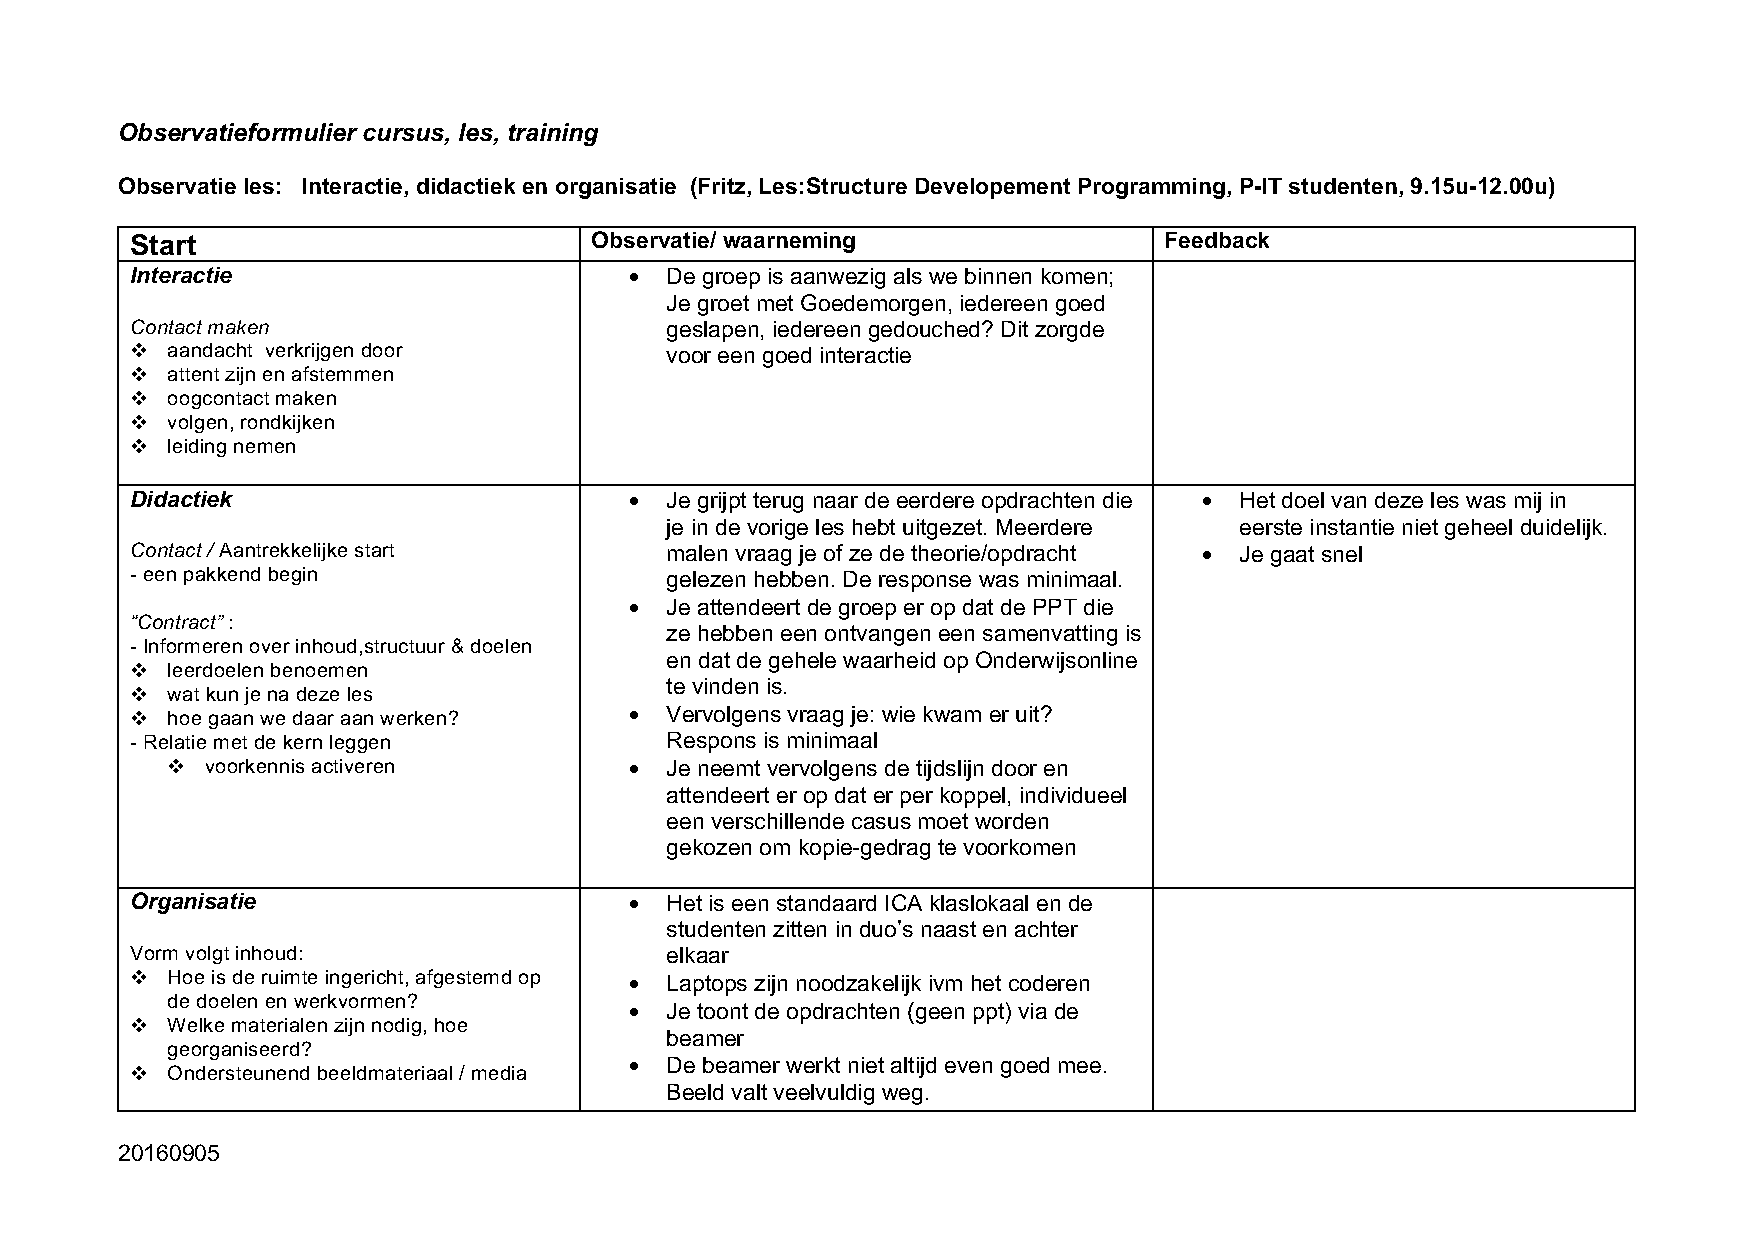
\includepdf[pages=-]{ObservatieCarmen.pdf}